\documentclass[aspectratio=169,10pt]{beamer}
\makeatletter
\def\input@path{{tuil_theme/}}
\makeatother
\def\titleimage{images/humbold.jpg}
\def\lastimage{images/campus.jpg}
\def\footercontent{\begin{tabular}{c|c|c}\insertshortauthor & Quantization study & \insertshorttitle\end{tabular}}
\usetheme{TUIl}
\usepackage{amsmath}
\usepackage{booktabs}
\usepackage{array}
\usepackage{graphicx}
\usepackage{tikz}
\usetikzlibrary{arrows.meta,positioning,shapes.geometric,fit,backgrounds,decorations.pathreplacing}
\graphicspath{{images/}{images/results/}}

\title[Neural-network quantization]{Analysis of Quantization Methods\\in Transformer-Based Neural Networks}
\author[S. Bhatt]{Sahil Bhatt}
\institute{Technische Universit\"at Ilmenau}
\date{23 September 2026}
\setbeamertemplate{navigation symbols}{}
\setlength{\tabcolsep}{4pt}
\setbeamerfont{block title}{size=\normalsize}

\tikzset{
  flow/.style={-{Latex[length=2.3mm]},line width=1.1pt,draw=TUIl-blue},
  floworange/.style={-{Latex[length=2.3mm]},line width=1.1pt,draw=TUIl-orange},
  card/.style={draw=TUIl-blue,rounded corners=2mm,fill=TUIl-blue!5,minimum height=10mm,align=center,inner sep=3mm},
  orangecard/.style={draw=TUIl-orange,rounded corners=2mm,fill=TUIl-orange!9,minimum height=10mm,align=center,inner sep=3mm},
  greencard/.style={draw=TUIl-green,rounded corners=2mm,fill=TUIl-green!9,minimum height=10mm,align=center,inner sep=3mm},
  process/.style={draw=TUIl-blue,rounded corners=1.2mm,fill=white,minimum width=21mm,minimum height=10mm,align=center,font=\small},
  neuron/.style={circle,draw=TUIl-blue,fill=TUIl-blue!12,minimum size=5.5mm,inner sep=0pt},
  tinylabel/.style={font=\scriptsize,align=center,text=TUIl-blue}
}
\newcommand{\takeaway}[1]{\vfill\begin{beamercolorbox}[wd=\textwidth,sep=1.5mm,rounded=true]{block body}\centering\small\bfseries #1\end{beamercolorbox}}

\begin{document}
\maketitle

\begin{frame}{Research questions and contribution}
\begin{columns}[T,onlytextwidth]
\column{.57\textwidth}
\begin{block}{Research questions}
\small
\begin{enumerate}
  \item How do bit width and method affect accuracy and estimated storage?
  \item How do the three saved checkpoints respond at W4 and W8?
  \item Which kernels, tensors or modules are most sensitive?
  \item Does a W8 sensitivity ranking transfer to W4?
\end{enumerate}
\end{block}
\column{.41\textwidth}
\begin{alertblock}{What was implemented}
\small
\begin{itemize}
  \item Two custom post-training weight quantizers
  \item 42 full-model sweep configurations
  \item W4/W8 isolated sensitivity analysis
  \item Saved predictions and permutation tests
\end{itemize}
\end{alertblock}
\end{columns}
\takeaway{The study compares complete checkpoint--quantizer configurations and does not isolate architecture as the cause.}
\end{frame}

\section{Motivation}
\begin{frame}{What is a neural network?}
\begin{center}
\resizebox{.82\textwidth}{!}{%
\begin{tikzpicture}[x=15mm,y=9mm]
  \node[card,minimum width=25mm,minimum height=25mm] (input) at (-2.2,1.5)
    {\large input data\\[-1mm]\scriptsize image, text, numbers};

  \foreach \y in {0,1,2,3} \node[neuron] (a\y) at (0,\y) {};
  \foreach \n/\y in {0/-0.5,1/0.5,2/1.5,3/2.5,4/3.5} \node[neuron,fill=TUIl-orange!18] (b\n) at (2,\y) {};
  \foreach \y in {0,1,2,3} \node[neuron,fill=TUIl-green!17] (c\y) at (4,\y) {};

  \foreach \i in {0,1,2,3}{\foreach \j in {0,1,2,3,4}{\draw[TUIl-grey!55,line width=.45pt] (a\i)--(b\j);}}
  \foreach \i in {0,1,2,3,4}{\foreach \j in {0,1,2,3}{\draw[TUIl-grey!55,line width=.45pt] (b\i)--(c\j);}}

  \draw[flow] (input.east)--(a1.west);
  \node[tinylabel,above=4mm of a3] {input layer};
  \node[tinylabel,above=4mm of b4] {hidden layer\\learned features};
  \node[tinylabel,above=4mm of c3] {output layer};

  \node[greencard,minimum width=25mm,minimum height=25mm] (output) at (6.3,1.5)
    {\large prediction\\[-1mm]\scriptsize class, score, value};
  \draw[flow] (c1.east)--(output.west);

  \node[orangecard,minimum width=45mm,minimum height=12mm] (learn) at (2,-2.0)
    {training adjusts connection weights\\to reduce prediction error};
  \draw[floworange,bend right=24] (output.south) to (learn.east);
  \draw[floworange,bend right=24] (learn.west) to (a0.south);
\end{tikzpicture}
}
\end{center}
\takeaway{A neural network learns weighted connections that transform input data into a useful prediction.}
\end{frame}



\section{Architectures}
\begin{frame}{What is a convolutional neural network?}
\begin{beamercolorbox}[wd=\textwidth,sep=1.5mm,rounded=true]{block body}
\small A CNN learns filters that slide across an image, detecting local patterns and combining them into higher-level features.
\end{beamercolorbox}
\vspace{1mm}
\centering
{\small\bfseries ResNet-18 used in this study}\par\vspace{1mm}
\resizebox{.89\textwidth}{!}{%
\begin{tikzpicture}[x=1cm,y=1cm,
  stage/.style={draw=TUIl-blue,fill=TUIl-blue!5,rounded corners=1.5mm,
    text width=28mm,minimum height=13mm,inner sep=2mm,align=center,font=\small},
  residual/.style={stage,draw=TUIl-orange,fill=TUIl-orange!9},
  output/.style={stage,draw=TUIl-green,fill=TUIl-green!9}]
  \node[stage] (image) at (0,0) {CIFAR-10 image\\$32\times32\times3$};
  \node[stage] (input) at (3.8,0) {Resize + preprocess\\$224\times224\times3$};
  \node[stage] (stem) at (7.6,0) {$7\times7$ convolution\\BatchNorm $\rightarrow$ ReLU};
  \node[stage] (pool) at (11.4,0) {$3\times3$ max pooling\\\scriptsize spatial downsampling};
  \draw[flow] (image)--(input);
  \draw[flow] (input)--(stem);
  \draw[flow] (stem)--(pool);

  \node[residual] (s0) at (11.4,-1.9) {\textbf{Stack 0}\\2 residual blocks\\64 channels};
  \node[residual] (s1) at (7.6,-1.9) {\textbf{Stack 1}\\2 residual blocks\\128 channels};
  \node[residual] (s2) at (3.8,-1.9) {\textbf{Stack 2}\\2 residual blocks\\256 channels};
  \node[residual] (s3) at (0,-1.9) {\textbf{Stack 3}\\2 residual blocks\\512 channels};
  \draw[floworange] (pool.south)--(s0.north);
  \draw[floworange] (s0)--(s1);
  \draw[floworange] (s1)--(s2);
  \draw[floworange] (s2)--(s3);
  \node[font=\scriptsize,text=TUIl-blue,align=center] at (5.7,-2.9)
    {Each residual block: two $3\times3$ convolutions + a shortcut};

  \node[stage] (gap) at (0,-3.9) {Global average\\pooling\\512 features};
  \node[stage] (dropout) at (5.7,-3.9) {Dropout: rate 0\\inactive};
  \node[output] (head) at (11.4,-3.9) {Dense classifier\\10 class scores};
  \draw[flow] (s3.south)--(gap.north);
  \draw[flow] (gap)--(dropout);
  \draw[flow] (dropout)--(head);
\end{tikzpicture}}
\end{frame}

\begin{frame}{ResNet-18: expanded stacks 0--3}
\centering
{\small Each stack contains two residual blocks; each convolution is followed by BatchNorm.}\par\vspace{2mm}
\resizebox{.93\textwidth}{!}{%
\begin{tikzpicture}[x=1cm,y=1cm,
  stacklabel/.style={text width=25mm,align=center,font=\small\bfseries,text=TUIl-blue},
  unit/.style={draw=TUIl-blue,fill=TUIl-blue!5,rounded corners=1mm,
    text width=42mm,minimum height=10mm,inner sep=1.5mm,align=center,font=\scriptsize},
  transition/.style={unit,draw=TUIl-orange,fill=TUIl-orange!9},
  dims/.style={text width=23mm,align=center,font=\scriptsize,text=TUIl-blue}]
  \node[stacklabel] at (0,0) {Stack 0\\64 channels};
  \node[unit] (a0) at (3.6,0) {\textbf{Block 0}\\$3\times3$: $64\to64$, stride 1\\$3\times3$: $64\to64$, stride 1\\Shortcut: identity};
  \node[unit] (a1) at (8.8,0) {\textbf{Block 1}\\$3\times3$: $64\to64$, stride 1\\$3\times3$: $64\to64$, stride 1\\Shortcut: identity};
  \node[dims] at (12.7,0) {$56\times56\times64$\\output};
  \draw[flow] (a0)--(a1);

  \node[stacklabel] at (0,-1.55) {Stack 1\\128 channels};
  \node[transition] (b0) at (3.6,-1.55) {\textbf{Block 0}\\$3\times3$: $64\to128$, stride 2\\$3\times3$: $128\to128$, stride 1\\Shortcut: $1\times1$, stride 2};
  \node[unit] (b1) at (8.8,-1.55) {\textbf{Block 1}\\$3\times3$: $128\to128$, stride 1\\$3\times3$: $128\to128$, stride 1\\Shortcut: identity};
  \node[dims] at (12.7,-1.55) {$28\times28\times128$\\output};
  \draw[flow] (b0)--(b1);

  \node[stacklabel] at (0,-3.10) {Stack 2\\256 channels};
  \node[transition] (c0) at (3.6,-3.10) {\textbf{Block 0}\\$3\times3$: $128\to256$, stride 2\\$3\times3$: $256\to256$, stride 1\\Shortcut: $1\times1$, stride 2};
  \node[unit] (c1) at (8.8,-3.10) {\textbf{Block 1}\\$3\times3$: $256\to256$, stride 1\\$3\times3$: $256\to256$, stride 1\\Shortcut: identity};
  \node[dims] at (12.7,-3.10) {$14\times14\times256$\\output};
  \draw[flow] (c0)--(c1);

  \node[stacklabel] at (0,-4.65) {Stack 3\\512 channels};
  \node[transition] (d0) at (3.6,-4.65) {\textbf{Block 0}\\$3\times3$: $256\to512$, stride 2\\$3\times3$: $512\to512$, stride 1\\Shortcut: $1\times1$, stride 2};
  \node[unit] (d1) at (8.8,-4.65) {\textbf{Block 1}\\$3\times3$: $512\to512$, stride 1\\$3\times3$: $512\to512$, stride 1\\Shortcut: identity};
  \node[dims] at (12.7,-4.65) {$7\times7\times512$\\output};
  \draw[flow] (d0)--(d1);
\end{tikzpicture}}
\par\vspace{1mm}{\scriptsize Block: Conv $\to$ BN $\to$ ReLU $\to$ Conv $\to$ BN $\to$ add shortcut $\to$ ReLU. Projection shortcuts also use BN.}
\end{frame}


\begin{frame}{What is a Transformer?}
\begin{beamercolorbox}[wd=\textwidth,sep=1.5mm,rounded=true]{block body}
\centering\small
A Transformer represents an input as a sequence of tokens, uses self-attention to exchange information between them, and transforms each token with a feed-forward network.
\end{beamercolorbox}
\vspace{1mm}
\centering
\resizebox{.96\textwidth}{!}{%
\begin{tikzpicture}[x=1cm,y=1cm,
  stage/.style={draw=TUIl-blue,fill=TUIl-blue!5,rounded corners=1.5mm,
    text width=20mm,minimum height=13mm,inner sep=1.5mm,align=center,font=\small},
  enc/.style={stage,draw=TUIl-orange,fill=TUIl-orange!9},
  result/.style={stage,draw=TUIl-green,fill=TUIl-green!9}]
  \node[stage] (text) at (0,.65) {Text\\\scriptsize subword tokens};
  \node[stage] (image) at (0,-.65) {Image\\\scriptsize patch tokens};
  \node[stage] (tokens) at (2.8,0) {Token / patch\\projection};
  \node[stage] (embed) at (5.6,0) {Embeddings\\$+$ positions};
  \node[enc,text width=25mm,minimum height=18mm] (stack) at (8.7,0)
    {\textbf{Transformer encoder stack}\\repeat the block below $N$ times};
  \node[stage] (context) at (11.8,0) {Contextual\\tokens};
  \node[result] (head) at (14.6,0) {[CLS] / pooling\\task head};
  \draw[flow] (text.east)--(tokens.west);
  \draw[flow] (image.east)--(tokens.west);
  \draw[flow] (tokens)--(embed);
  \draw[floworange] (embed)--(stack);
  \draw[floworange] (stack)--(context);
  \draw[flow] (context)--(head);

  \node[font=\small\bfseries,text=TUIl-blue] at (0,-2.25) {One encoder block};
  \node[stage,text width=17mm] (xin) at (2.5,-2.25) {Input sequence\\$X$};
  \node[enc,text width=19mm] (attn) at (5.2,-2.25) {LayerNorm\\multi-head\\self-attention};
  \node[stage,text width=18mm] (add1) at (7.9,-2.25) {Add residual\\$X+$ attention};
  \node[enc,text width=19mm] (ffn) at (10.6,-2.25) {LayerNorm\\feed-forward\\network};
  \node[result,text width=18mm] (add2) at (13.3,-2.25) {Add residual\\block output};
  \draw[floworange] (xin)--(attn);
  \draw[floworange] (attn)--(add1);
  \draw[floworange] (add1)--(ffn);
  \draw[floworange] (ffn)--(add2);
\end{tikzpicture}}
\par\vspace{1mm}{\tiny Text uses subword tokens; vision uses image-patch tokens. Both use the same encoder computation.\hfill Vaswani et al., 2017}
\end{frame}

\begin{frame}{What is DistilBERT?}
\begin{beamercolorbox}[wd=\textwidth,sep=1.5mm,rounded=true]{block body}
\small DistilBERT is a smaller version of BERT learned through knowledge distillation. Its six encoder blocks build contextual text representations for tasks such as sentiment classification.
\end{beamercolorbox}
\vspace{1mm}
\centering
\resizebox{.95\textwidth}{!}{%
\begin{tikzpicture}[x=1cm,y=1cm,
  stage/.style={draw=TUIl-blue,fill=TUIl-blue!5,rounded corners=1.5mm,
    text width=25mm,minimum height=14mm,inner sep=1.5mm,align=center,font=\small},
  encoder/.style={stage,text width=19mm,draw=TUIl-orange,fill=TUIl-orange!9},
  output/.style={stage,draw=TUIl-green,fill=TUIl-green!9}]
  \node[stage] (sentence) at (0,0) {Input sentence};
  \node[stage] (tokenizer) at (3.2,0) {Tokenizer\\+ special tokens\\+ padding mask};
  \node[stage] (ids) at (6.4,0) {128 token IDs};
  \node[stage] (embed) at (9.6,0) {Token\\embeddings\\+ position\\embeddings};
  \node[stage] (norm) at (12.8,0) {Layer\\normalization\\+ dropout};
  \draw[flow] (sentence)--(tokenizer);
  \draw[flow] (tokenizer)--(ids);
  \draw[flow] (ids)--(embed);
  \draw[flow] (embed)--(norm);

  \node[encoder] (b0) at (12.8,-1.9) {Transformer\\encoder\\\textbf{block 0}};
  \node[encoder] (b1) at (10.24,-1.9) {Transformer\\encoder\\\textbf{block 1}};
  \node[encoder] (b2) at (7.68,-1.9) {Transformer\\encoder\\\textbf{block 2}};
  \node[encoder] (b3) at (5.12,-1.9) {Transformer\\encoder\\\textbf{block 3}};
  \node[encoder] (b4) at (2.56,-1.9) {Transformer\\encoder\\\textbf{block 4}};
  \node[encoder] (b5) at (0,-1.9) {Transformer\\encoder\\\textbf{block 5}};
  \draw[floworange] (norm.south)--(b0.north);
  \draw[floworange] (b0)--(b1);
  \draw[floworange] (b1)--(b2);
  \draw[floworange] (b2)--(b3);
  \draw[floworange] (b3)--(b4);
  \draw[floworange] (b4)--(b5);

  \node[stage] (cls) at (0,-3.8) {Final [CLS]\\representation\\768 features};
  \node[stage] (projection) at (3.2,-3.8) {Dense projection\\$768\rightarrow768$\\ReLU};
  \node[stage] (dropout) at (6.4,-3.8) {Classifier\\dropout};
  \node[stage] (classifier) at (9.6,-3.8) {Dense classifier\\$768\rightarrow2$};
  \node[output] (scores) at (12.8,-3.8) {Negative /\\positive\\class scores};
  \draw[flow] (b5.south)--(cls.north);
  \draw[flow] (cls)--(projection);
  \draw[flow] (projection)--(dropout);
  \draw[flow] (dropout)--(classifier);
  \draw[flow] (classifier)--(scores);
\end{tikzpicture}}
\par\vspace{1mm}{\scriptsize SST-2: 872 evaluation examples; 88.42\% FP32 accuracy.\hfill Sanh et al., 2019}
\end{frame}

\begin{frame}{What is ViT-B/16?}
\begin{beamercolorbox}[wd=\textwidth,sep=1.5mm,rounded=true]{block body}
\small ViT-B/16 is a Vision Transformer that converts an image into $16\!\times\!16$-pixel patch tokens and processes them with 12 Transformer encoder blocks for image classification.
\end{beamercolorbox}
\vspace{1mm}
\centering
\resizebox{.95\textwidth}{!}{%
\begin{tikzpicture}[x=1cm,y=1cm,
  stage/.style={draw=TUIl-blue,fill=TUIl-blue!5,rounded corners=1.5mm,
    text width=25mm,minimum height=14mm,inner sep=1.5mm,align=center,font=\small},
  encoder/.style={stage,text width=17mm,draw=TUIl-orange,fill=TUIl-orange!9},
  output/.style={stage,draw=TUIl-green,fill=TUIl-green!9}]
  \node[stage] (image) at (0,0) {Input image\\$224\!\times\!224\!\times\!3$};
  \node[stage] (patches) at (3.2,0) {Split into\\$16\!\times\!16$ patches\\$14\!\times\!14=196$};
  \node[stage] (projection) at (6.4,0) {Flatten + linear\\projection\\$768$ features};
  \node[stage] (tokens) at (9.6,0) {Prepend learned\\{[CLS]} token\\197 tokens};
  \node[stage] (positions) at (12.8,0) {Add position\\embeddings\\+ dropout};
  \draw[flow] (image)--(patches);
  \draw[flow] (patches)--(projection);
  \draw[flow] (projection)--(tokens);
  \draw[flow] (tokens)--(positions);

  \node[encoder] (b0) at (12.8,-1.8) {Encoder\\\textbf{blocks 0--1}};
  \node[encoder] (b1) at (10.24,-1.8) {Encoder\\\textbf{blocks 2--3}};
  \node[encoder] (b2) at (7.68,-1.8) {Encoder\\\textbf{blocks 4--5}};
  \node[encoder] (b3) at (5.12,-1.8) {Encoder\\\textbf{blocks 6--7}};
  \node[encoder] (b4) at (2.56,-1.8) {Encoder\\\textbf{blocks 8--9}};
  \node[encoder] (b5) at (0,-1.8) {Encoder\\\textbf{blocks 10--11}};
  \draw[floworange] (positions.south)--(b0.north);
  \draw[floworange] (b0)--(b1);
  \draw[floworange] (b1)--(b2);
  \draw[floworange] (b2)--(b3);
  \draw[floworange] (b3)--(b4);
  \draw[floworange] (b4)--(b5);

  \node[stage] (norm) at (0,-3.6) {Final layer\\normalization};
  \node[stage] (cls) at (3.2,-3.6) {Take final [CLS]\\representation\\768 features};
  \node[stage] (head) at (6.4,-3.6) {Dense classifier\\$768\rightarrow10$};
  \node[output] (scores) at (9.6,-3.6) {Ten CIFAR-10\\class scores};
  \draw[flow] (b5.south)--(norm.north);
  \draw[flow] (norm)--(cls);
  \draw[flow] (cls)--(head);
  \draw[flow] (head)--(scores);
\end{tikzpicture}}
\par\vspace{1mm}{\scriptsize CIFAR-10: 10,000 test images; 95.73\% FP32 accuracy.\hfill Dosovitskiy et al., 2021}
\end{frame}

\section{Quantization}
\begin{frame}{What is quantization?}
\begin{beamercolorbox}[wd=\textwidth,sep=2.5mm,rounded=true]{block body}
\centering\large
Quantization represents high-precision neural-network values with a smaller set of low-bit discrete values.
\end{beamercolorbox}
\vspace{2mm}
\begin{columns}[T,onlytextwidth]
\column{.305\textwidth}
\begin{block}{What changes?}
\centering\small
FP32 weights are approximated using $b$-bit values.
\end{block}
\column{.305\textwidth}
\begin{block}{Why use it?}
\centering\small
Fewer bits reduce model storage and memory traffic.
\end{block}
\column{.305\textwidth}
\begin{block}{What is the cost?}
\centering\small
Rounding introduces error that may reduce accuracy.
\end{block}
\end{columns}
\vspace{2mm}
\begin{alertblock}{Scope of this study}
\centering\small
Both custom methods are post-training and weight-only, with no quantization-aware training.\\
\scriptsize Estimated packed parameter storage; accuracy evaluated using FP32-reconstructed weights and FP32 activations.
\end{alertblock}
\takeaway{The objective is to reduce the bits per weight while retaining as much FP32 accuracy as possible.}
\end{frame}

\begin{frame}{Uniform PTQ: method and implementation}
\begin{beamercolorbox}[wd=\textwidth,sep=1.7mm,rounded=true]{block body}
\small Uniform post-training quantization maps trained FP32 weights to an evenly spaced low-bit grid after training, without gradient updates or retraining.
\par\vspace{.3mm}{\raggedleft\tiny Jacob et al., 2018\par}
\end{beamercolorbox}
\vspace{1mm}
\centering
\resizebox{.93\textwidth}{!}{%
\begin{tikzpicture}[x=1cm,y=1cm,
  ptqbox/.style={draw=TUIl-blue,fill=TUIl-blue!5,rounded corners=1.5mm,
    text width=25mm,minimum height=18mm,inner sep=1.5mm,align=center,font=\small},
  qstep/.style={ptqbox,draw=TUIl-orange,fill=TUIl-orange!9},
  result/.style={ptqbox,draw=TUIl-green,fill=TUIl-green!9}]
  \node[ptqbox] (tensor) at (0,0) {Select an FP32\\weight tensor $W$};
  \node[ptqbox] (channel) at (3.1,0) {Split by output\\channel $W_c$};
  \node[qstep] (scale) at (6.2,0) {Find one scale\\per channel\\$s_c=\dfrac{\max|W_c|}{2^{b-1}-1}$};
  \node[qstep] (integer) at (9.3,0) {Divide, round, clip\\$q_c=\operatorname{clip}(\operatorname{round}(W_c/s_c))$};
  \node[result] (reconstruct) at (12.4,0) {Reconstruct weights\\$\widehat W_c=s_cq_c$};
  \draw[flow] (tensor)--(channel);
  \draw[flow] (channel)--(scale);
  \draw[floworange] (scale)--(integer);
  \draw[floworange] (integer)--(reconstruct);
\end{tikzpicture}}
\vspace{2mm}
\begin{columns}[T,onlytextwidth]
\column{.475\textwidth}
\begin{block}{Configuration used here}
\centering\scriptsize
$b=2,3,\ldots,8$; signed symmetric grid;\\
$2^b-1$ levels; per-output-channel scales.
\end{block}
\column{.475\textwidth}
\begin{block}{How it was evaluated}
\centering\scriptsize
Weight-only simulated PTQ: reconstructed weights and FP32 activations were used for accuracy evaluation.
\end{block}
\end{columns}
\takeaway{Each weight is replaced by its nearest available grid value; lower bit widths create a coarser approximation.}
\end{frame}

\begin{frame}{Codebook quantization: how it works}
\begin{beamercolorbox}[wd=\textwidth,sep=1.6mm,rounded=true]{block body}
\small Codebook quantization learns $K=2^b$ representative weight values, called centroids, and replaces every FP32 weight with the index of its nearest centroid.
\par\vspace{.3mm}{\raggedleft\tiny Gray, 1984; Lloyd, 1982\par}
\end{beamercolorbox}
\vspace{1mm}
\centering
\resizebox{.94\textwidth}{!}{%
\begin{tikzpicture}[x=1cm,y=1cm,
  cbbox/.style={draw=TUIl-blue,fill=TUIl-blue!5,rounded corners=1.5mm,
    text width=25mm,minimum height=17mm,inner sep=1.2mm,align=center,font=\small},
  learn/.style={cbbox,draw=TUIl-orange,fill=TUIl-orange!9},
  result/.style={cbbox,draw=TUIl-green,fill=TUIl-green!9}]
  \node[cbbox] (tensor) at (0,0) {Flatten the selected\\FP32 tensor $W$};
  \node[learn] (initial) at (3.15,0) {Set $K=2^b$ and\\initialize $K$ centroids};
  \node[learn] (assign) at (6.3,0) {Assign nearest centroid\\[-1mm]\scriptsize $q(w)=\arg\min_k|w-c_k|$};
  \node[learn] (update) at (9.45,0) {Update each centroid\\to its cluster's mean};
  \node[cbbox] (repeat) at (12.6,0) {Repeat assignment\\and update until stable};
  \draw[flow] (tensor)--(initial);
  \draw[floworange] (initial)--(assign);
  \draw[floworange] (assign)--(update);
  \draw[floworange] (update)--(repeat);

  \node[cbbox,text width=39mm,minimum height=12mm] (index) at (10.3,-1.75)
    {Store one $b$-bit centroid index\\for each weight};
  \node[result,text width=39mm,minimum height=12mm] (reconstruct) at (5.0,-1.75)
    {Reconstruct each weight\\$\widehat w=c_{q(w)}$ for evaluation};
  \draw[flow] (repeat.south)--(index.north);
  \draw[flow] (index)--(reconstruct);
\end{tikzpicture}}
\vspace{1mm}
\begin{beamercolorbox}[wd=\textwidth,sep=1.2mm,rounded=true]{block body}
\centering\scriptsize Cluster means follow the tensor's weight distribution, so the learned centroid levels are generally unevenly spaced.
\end{beamercolorbox}
\takeaway{The codebook contains the centroid values; the quantized tensor contains their indices.}
\end{frame}

\begin{frame}{Experimental methodology: tensor selection}
\begin{center}
\resizebox{.85\textwidth}{!}{%
\begin{tikzpicture}[node distance=7mm]
  \node[card,minimum width=28mm] (all) {ordered FP32\\model weights};
  \node[process,right=of all,minimum width=29mm] (eligible) {floating point\\and rank $\geq2$};
  \node[orangecard,right=of eligible,minimum width=31mm] (filter) {apply model-specific\\path filter};
  \node[greencard,right=of filter,minimum width=29mm] (selected) {selected weights\\quantized};
  \draw[flow] (all)--(eligible);
  \draw[flow] (eligible)--(filter);
  \draw[floworange] (filter)--(selected);
  \node[tinylabel,below=3mm of filter] {same selection for PTQ and codebook};
\end{tikzpicture}
}
\end{center}
\vspace{1mm}
\begin{columns}[T,onlytextwidth]
\column{.305\textwidth}
\begin{block}{ResNet-18: 21}
\centering\scriptsize
All floating tensors with rank $\geq2$\\[1mm]
Convolution and classifier kernels
\end{block}
\column{.305\textwidth}
\begin{block}{DistilBERT: 40}
\centering\scriptsize
Paths ending in \texttt{/kernel} or \texttt{/embeddings}\\[1mm]
Token/position embeddings; Q, K, V and attention-output kernels; both feed-forward kernels; pooled and classifier kernels
\end{block}
\column{.305\textwidth}
\begin{block}{ViT-B/16: 76}
\centering\scriptsize
Paths ending in \texttt{/kernel} or \texttt{/embeddings}, plus \texttt{class\_token}\\[1mm]
Patch/position embeddings; six kernels in each of 12 blocks; classifier kernel
\end{block}
\end{columns}
\vspace{1mm}
\begin{center}\scriptsize For sensitivity analysis, the 76 ViT tensors are grouped into 14 logical modules; seven predefined modules are tested at W4.\end{center}
\begin{beamercolorbox}[wd=\textwidth,sep=1mm,rounded=true]{block body}\centering\scriptsize\bfseries
No bias tensors were selected; rank-one biases, normalization scale/offset vectors and rank-two attention biases remained FP32.
\end{beamercolorbox}
\end{frame}

\section{Methodology}
\begin{frame}{Evaluated checkpoints and datasets}
\begin{center}
\renewcommand{\arraystretch}{1.65}
\setlength{\tabcolsep}{3.2pt}
\small
\begin{tabular}{>{\bfseries}l l c r r r}
\toprule
Model & Dataset & Examples & Parameters & FP32 size & Accuracy\\
\midrule
ResNet-18 & CIFAR-10 test & 10,000 & 11.19 M & 42.69 MiB & 90.47\%\\
DistilBERT & SST-2 dev & 872 & 66.96 M & 255.41 MiB & 88.42\%\\
ViT-B/16 & CIFAR-10 test & 10,000 & 85.81 M & 327.33 MiB & 95.73\%\\
\bottomrule
\end{tabular}
\end{center}
\vspace{3mm}
\begin{columns}[T,onlytextwidth]
\column{.305\textwidth}\begin{block}{ResNet-18}\centering\scriptsize Adapted end-to-end\end{block}
\column{.305\textwidth}\begin{block}{DistilBERT}\centering\scriptsize Fine-tuned for SST-2\end{block}
\column{.305\textwidth}\begin{block}{ViT-B/16}\centering\scriptsize Backbone frozen; head trained\end{block}
\end{columns}
\takeaway{Every quantized result is compared with the FP32 accuracy of the same saved checkpoint.}
\end{frame}

\begin{frame}{Experimental methodology: experiment map}
\begin{center}
\resizebox{.95\textwidth}{!}{%
\begin{tikzpicture}[node distance=5mm]
  \node[card,minimum width=18mm] (e1) {1\\FP32\\baseline};
  \node[process,right=of e1,minimum width=19mm] (e2) {2\\built-in W8\\check};
  \node[orangecard,right=of e2,minimum width=19mm] (e3) {3\\full model\\W2--W8};
  \node[process,right=of e3,minimum width=21mm] (e4) {4\\one analysis unit\\at a time};
  \node[process,right=of e4,minimum width=21mm] (e5) {5\\W4/W8 rank\\stability};
  \draw[flow] (e1)--(e2); \draw[flow] (e2)--(e3); \draw[flow] (e3)--(e4); \draw[flow] (e4)--(e5);
  \node[tinylabel,below=5mm of e1] {reference};
  \node[tinylabel,below=5mm of e3] {accuracy / storage};
  \node[tinylabel,below=5mm of e4] {sensitivity maps};
  \node[tinylabel,below=5mm of e5] {answers RQ4};
\end{tikzpicture}
}
\end{center}
\vspace{2mm}
\begin{columns}[T,onlytextwidth]
\column{.475\textwidth}\begin{block}{Full-model tensors}\centering\small ResNet: 21 \quad DistilBERT: 40 \quad ViT: 76\end{block}
\column{.475\textwidth}\begin{block}{Isolated sensitivity}\centering\small W8: exhaustive \quad W4: 21 kernels / 15 tensors / 7 modules\end{block}
\end{columns}
\takeaway{The sweep measures system behavior; isolated replacement locates which weights drive it.}
\end{frame}

\begin{frame}{Baseline checks}
\vfill
\begin{center}
\renewcommand{\arraystretch}{1.8}
\setlength{\tabcolsep}{7pt}
\resizebox{.92\textwidth}{!}{%
\begin{tabular}{l l r r r}
\toprule
Model & Built-in path & FP32 & Built-in W8 & Compression\\
\midrule
ResNet-18 & Full INT8, W8A8 & 90.47\% & 88.53\% & $4.00\times$\\
DistilBERT & \shortstack[l]{TFLite dynamic-range\\quantization} & 88.42\% & 88.07\% & $3.99\times$\\
ViT-B/16 & \shortstack[l]{TFLite dynamic-range\\quantization} & 95.73\% & 95.78\% & $3.96\times$\\
\bottomrule
\end{tabular}%
}
\end{center}
\vfill
\end{frame}

\begin{frame}{Custom PTQ: full W2--W8 sweep}
\centering
\scriptsize $A$: accuracy (\%) \qquad $R$: compression ratio ($\times$) \qquad $S$: parameter-memory reduction (\%)
\vspace{1mm}

\resizebox{.94\textwidth}{!}{%
\renewcommand{\arraystretch}{1.15}
\begin{tabular}{c rrr rrr rrr}
\toprule
& \multicolumn{3}{c}{\textbf{ResNet-18}} & \multicolumn{3}{c}{\textbf{DistilBERT}} & \multicolumn{3}{c}{\textbf{ViT-B/16}}\\
Bits & $A$ & $R$ & $S$ & $A$ & $R$ & $S$ & $A$ & $R$ & $S$\\
\midrule
2 & 10.00 & 15.60 & 93.59 & 51.03 & 15.67 & 93.62 & 13.00 & 15.50 & 93.55\\
3 & 11.23 & 10.49 & 90.47 & 82.91 & 10.52 & 90.49 & 32.22 & 10.45 & 90.43\\
4 & 11.56 & 7.91 & 87.35 & 88.99 & 7.92 & 87.37 & 95.23 & 7.88 & 87.31\\
5 & 49.39 & 6.34 & 84.23 & 88.19 & 6.35 & 84.25 & 95.83 & 6.32 & 84.19\\
6 & 71.87 & 5.29 & 81.11 & 88.07 & 5.30 & 81.13 & 95.70 & 5.28 & 81.06\\
7 & 88.05 & 4.54 & 77.99 & 88.30 & 4.55 & 78.01 & 95.75 & 4.53 & 77.94\\
8 & 89.88 & 3.98 & 74.87 & 88.42 & 3.98 & 74.88 & 95.79 & 3.97 & 74.82\\
\bottomrule
\end{tabular}%
}\par
\vspace{1mm}\scriptsize Estimated packed parameter storage; accuracy uses FP32-reconstructed weights.
\end{frame}

\begin{frame}{Scalar codebook: full W2--W8 sweep}
\centering
\scriptsize $A$: accuracy (\%) \qquad $R$: compression ratio ($\times$) \qquad $S$: parameter-memory reduction (\%)
\vspace{1mm}

\resizebox{.90\textwidth}{!}{%
\renewcommand{\arraystretch}{1.15}
\begin{tabular}{c rrr rrr rrr}
\toprule
& \multicolumn{3}{c}{\textbf{ResNet-18}} & \multicolumn{3}{c}{\textbf{DistilBERT}} & \multicolumn{3}{c}{\textbf{ViT-B/16}}\\
Bits & $A$ & $R$ & $S$ & $A$ & $R$ & $S$ & $A$ & $R$ & $S$\\
\midrule
2 & 9.50 & 15.60 & 93.59 & 78.33 & 15.78 & 93.66 & 20.84 & 15.66 & 93.62\\
3 & 10.00 & 10.49 & 90.47 & 86.24 & 10.57 & 90.54 & 89.77 & 10.52 & 90.50\\
4 & 8.43 & 7.90 & 87.35 & 88.30 & 7.95 & 87.42 & 95.20 & 7.92 & 87.37\\
5 & 15.41 & 6.34 & 84.22 & 88.19 & 6.37 & 84.29 & 95.64 & 6.35 & 84.25\\
6 & 48.71 & 5.29 & 81.10 & 88.07 & 5.31 & 81.17 & 95.76 & 5.30 & 81.13\\
7 & 88.97 & 4.54 & 77.97 & 88.42 & 4.55 & 78.04 & 95.68 & 4.55 & 78.00\\
8 & 90.25 & 3.97 & 74.82 & 88.07 & 3.99 & 74.92 & 95.73 & 3.98 & 74.87\\
\bottomrule
\end{tabular}%
}\par
\vspace{1mm}\scriptsize Estimated packed parameter storage; accuracy uses FP32-reconstructed weights.
\end{frame}

\section{Results}
\begin{frame}{Results: custom PTQ accuracy sweep}
\begin{columns}[c,onlytextwidth]
\column{.74\textwidth}
\centering
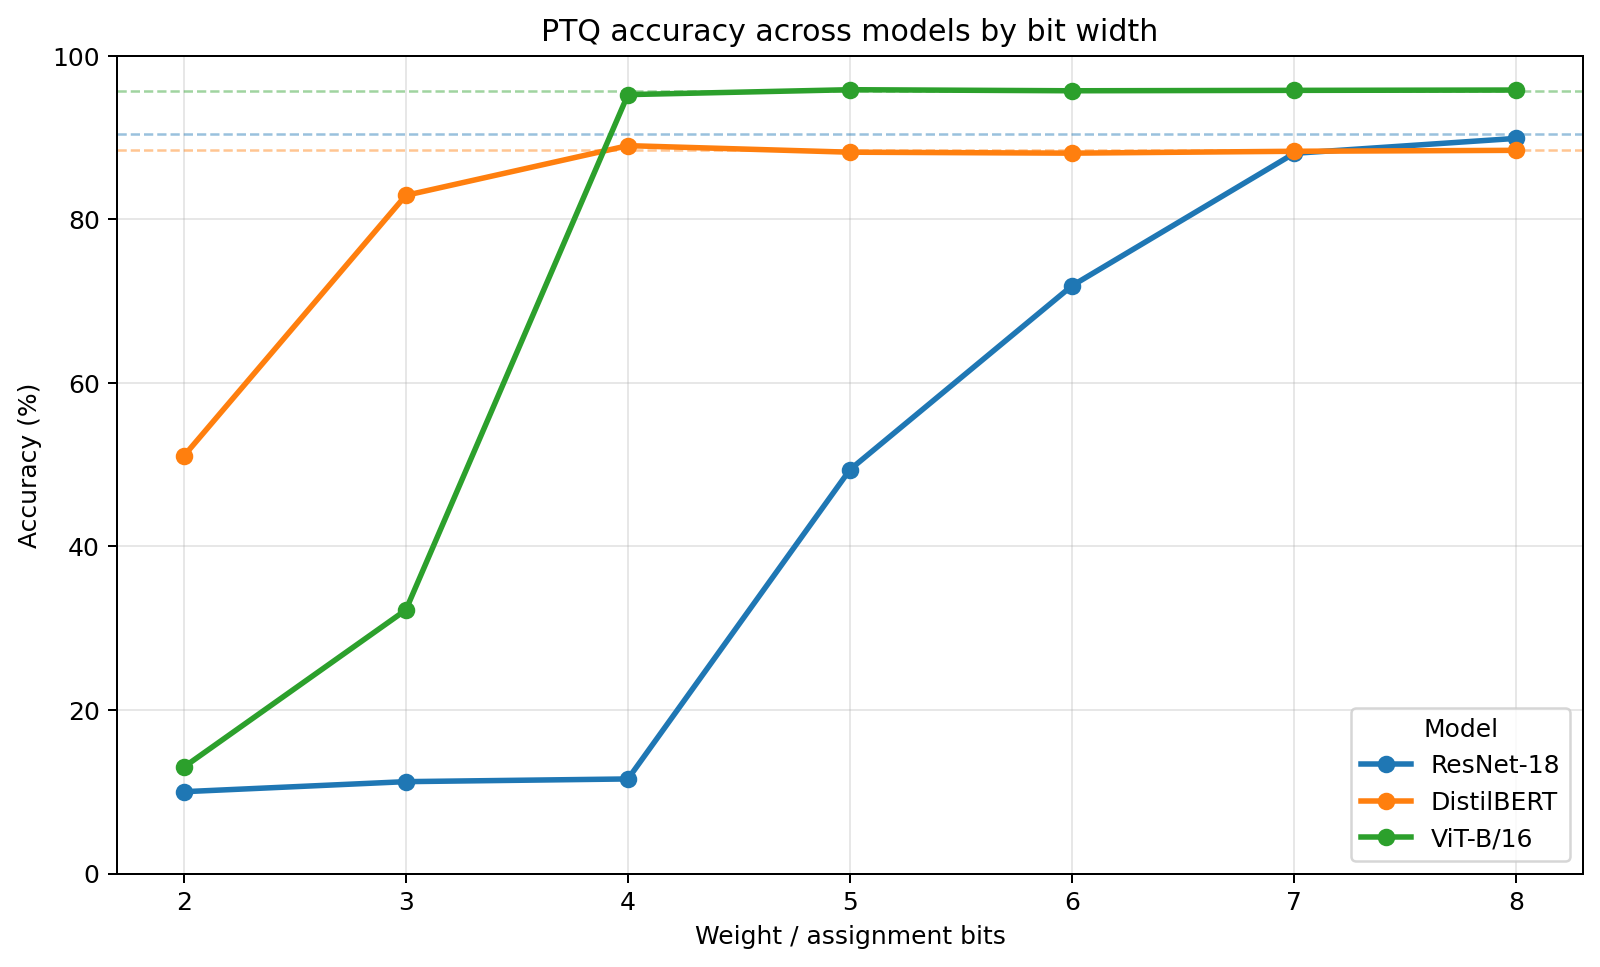
\includegraphics[width=\linewidth,height=.68\textheight,keepaspectratio]{ptq_accuracy_all_models_2_to_8_bit.png}
\column{.24\textwidth}
\begin{block}{At W4}
\centering\small
ResNet-18\\\textbf{11.56\%}\\[2mm]
DistilBERT\\\textbf{88.99\%}\\[2mm]
ViT-B/16\\\textbf{95.23\%}
\end{block}
\begin{alertblock}{Observed transition}
\centering\scriptsize ResNet recovers near W7; both transformer checkpoints recover at W4.
\end{alertblock}
\end{columns}
\end{frame}

\begin{frame}{Comparison: custom codebook accuracy sweep}
\begin{columns}[c,onlytextwidth]
\column{.74\textwidth}
\centering
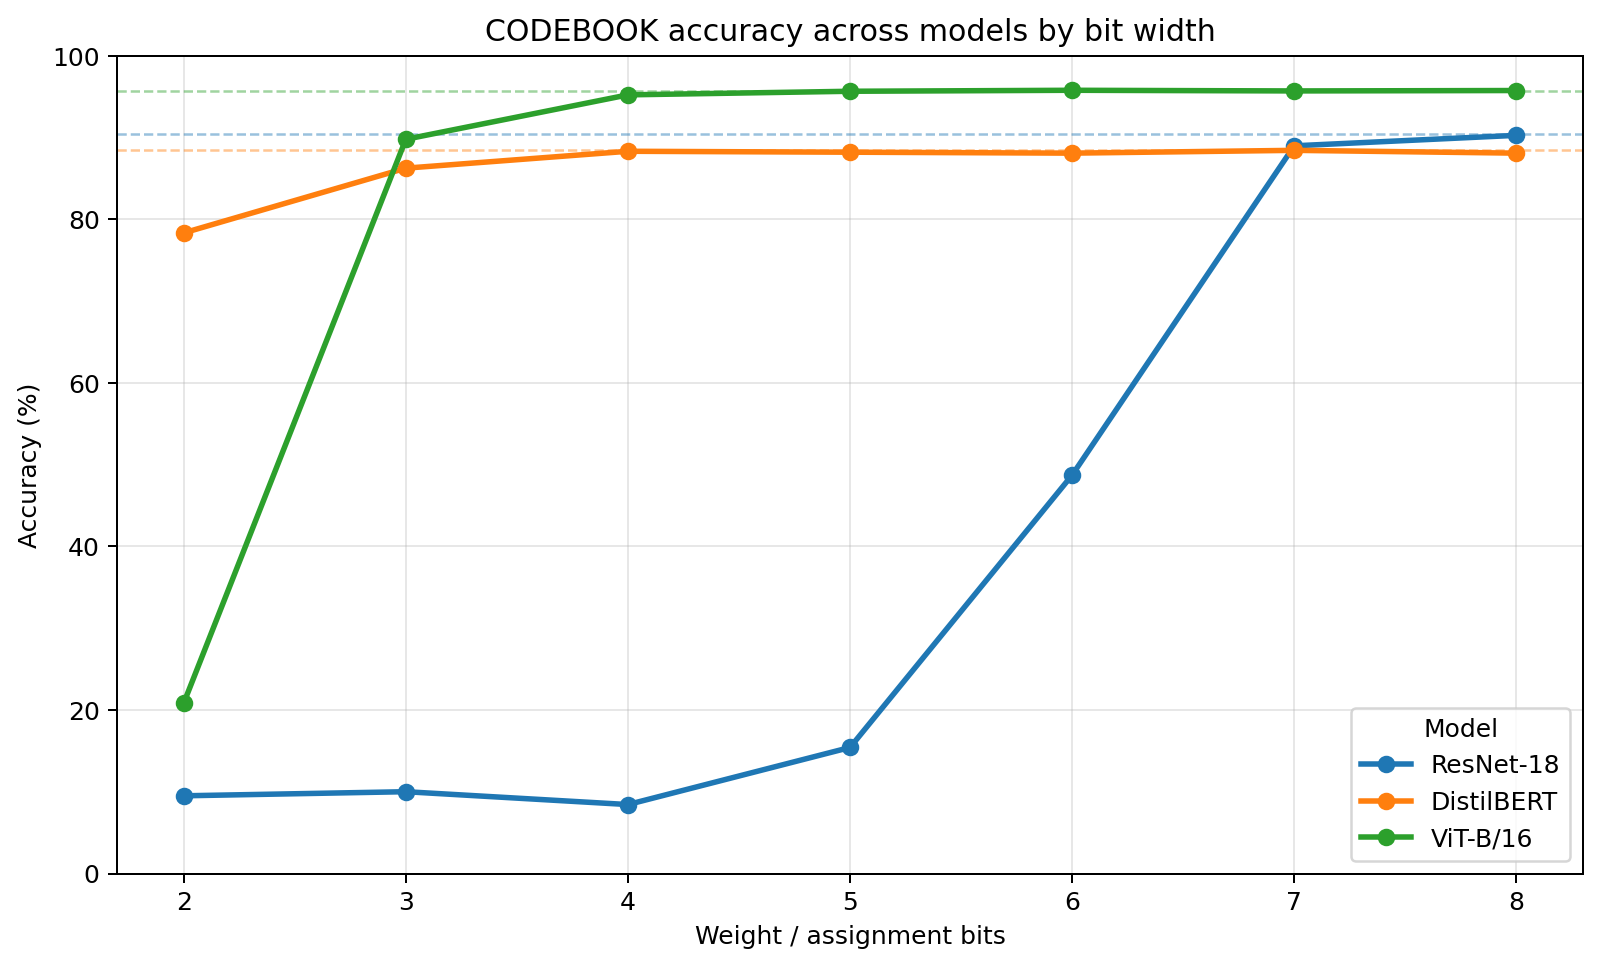
\includegraphics[width=\linewidth,height=.68\textheight,keepaspectratio]{codebook_accuracy_all_models_2_to_8_bit.png}
\column{.24\textwidth}
\begin{block}{Low-bit retention}
\centering\small
DistilBERT W2\\\textbf{78.33\%}\\[2mm]
ViT-B/16 W3\\\textbf{89.77\%}\\[2mm]
ResNet-18 W4\\\textbf{8.43\%}
\end{block}
\begin{alertblock}{Method contrast}
\centering\scriptsize Largest observed gap: ViT W3, codebook exceeds PTQ by 57.55 pp. The configurations also differ in granularity and level count.
\end{alertblock}
\end{columns}
\end{frame}

\begin{frame}{Accuracy and storage trade-off}
\begin{columns}[T,onlytextwidth]
\column{.305\textwidth}\centering
\textbf{ResNet-18}\par\vspace{1mm}
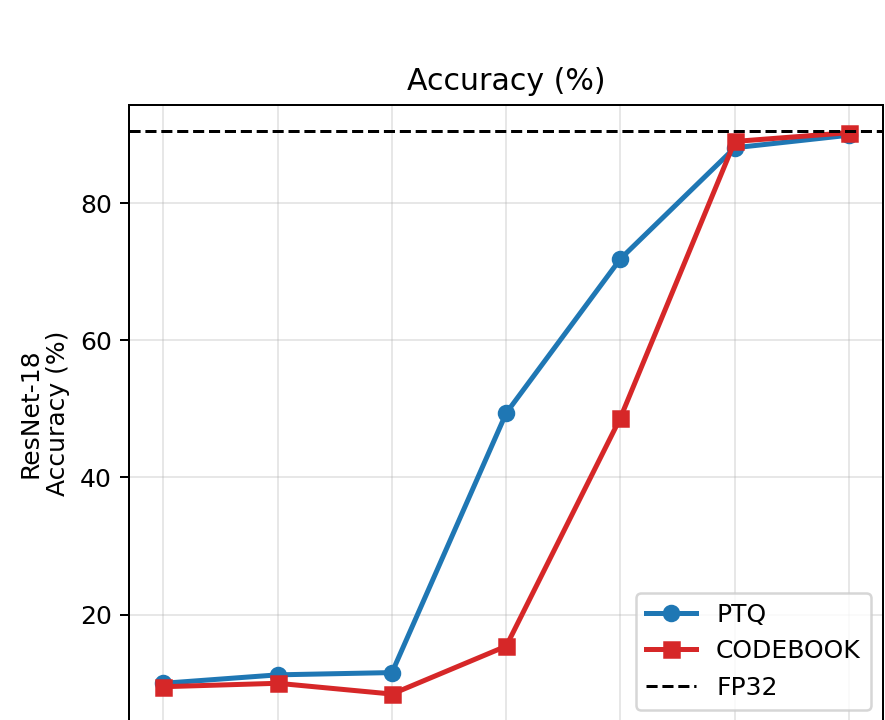
\includegraphics[width=\linewidth,height=.36\textheight,keepaspectratio]{notebook25_resnet_accuracy_panel.png}
\column{.305\textwidth}\centering
\textbf{DistilBERT}\par\vspace{1mm}
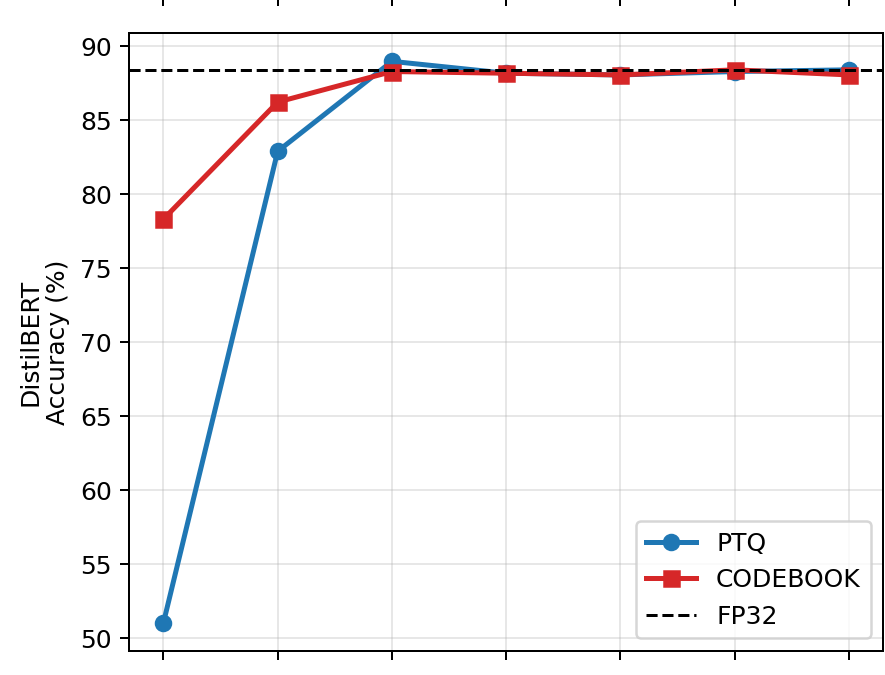
\includegraphics[width=\linewidth,height=.36\textheight,keepaspectratio]{notebook25_distilbert_accuracy_panel.png}
\column{.305\textwidth}\centering
\textbf{ViT-B/16}\par\vspace{1mm}
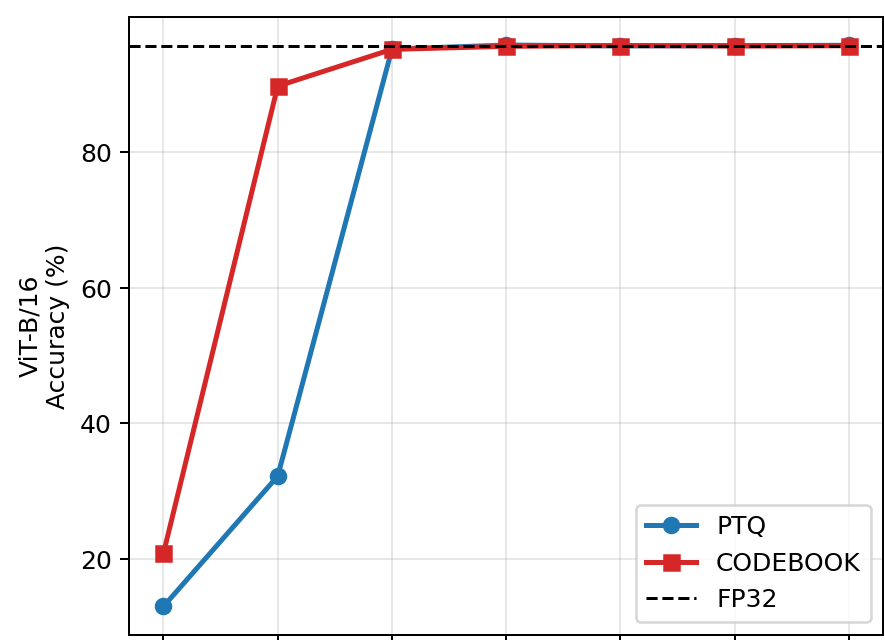
\includegraphics[width=\linewidth,height=.36\textheight,keepaspectratio]{notebook25_vit_accuracy_panel.png}
\end{columns}
\vspace{1mm}
\begin{columns}[c,onlytextwidth]
\column{.58\textwidth}
\begin{block}{Storage is mainly bit-width-driven}
\centering\scriptsize
\begin{tabular}{rcc}
\toprule
Bits & Compression & Reduction\\
\midrule
2 & $15.5$--$15.8\times$ & $93.6\%$\\
4 & $7.9\times$ & $87.3$--$87.4\%$\\
8 & $4.0\times$ & $74.8$--$74.9\%$\\
\bottomrule
\end{tabular}
\par\vspace{1mm}\scriptsize Estimated packed parameter storage.
\end{block}
\column{.40\textwidth}
\begin{alertblock}{One storage result, two views}
\centering\scriptsize
$S=100\left(1-1/R\right)$\\[1mm]
\scriptsize Memory reduction $S$ and compression ratio $R$ are mathematically linked.
\par\vspace{1mm}\scriptsize Accuracy uses FP32-reconstructed weights.
\end{alertblock}
\end{columns}
\end{frame}

\begin{frame}{Layer-by-layer comparison}
\begin{center}
\resizebox{.92\textwidth}{!}{%
\begin{tikzpicture}[node distance=8mm]
  \node[card,minimum width=31mm] (fp) {Start from the\\FP32 checkpoint};
  \node[process,right=of fp,minimum width=37mm] (one) {Quantize exactly one\\analysis unit};
  \node[process,right=of one,minimum width=31mm] (eval) {Evaluate the full\\labelled split};
  \node[orangecard,right=of eval,minimum width=34mm] (drop) {$\Delta A_u=A_{\mathrm{FP32}}-A_u$\\rank by degradation};
  \draw[flow] (fp)--(one); \draw[flow] (one)--(eval); \draw[floworange] (eval)--(drop);
\end{tikzpicture}}
\end{center}
\vspace{3mm}
\begin{columns}[T,onlytextwidth]
\column{.55\textwidth}
\begin{block}{Controlled comparison}
\small Every run restores the original checkpoint and leaves all other weights in FP32. Positive $\Delta A_u$ is an accuracy loss; a negative value is an observed gain.
\end{block}
\column{.43\textwidth}
\centering\scriptsize
\begin{tabular}{lccc}
\toprule
Model & Unit & W8 & W4\\
\midrule
ResNet-18 & kernel & 21/21 & 21/21\\
DistilBERT & tensor & 40/40 & 15/40\\
ViT-B/16 & module & 14/14 & 7/14\\
\bottomrule
\end{tabular}
\vspace{2mm}

\scriptsize Heatmaps: red = loss, blue = observed gain.
\end{columns}
\takeaway{This experiment locates vulnerable units; it does not measure interactions between several quantized units.}
\end{frame}

\begin{frame}{ResNet-18: layer sensitivity}
\begin{columns}[c,onlytextwidth]
\column{.48\textwidth}\centering
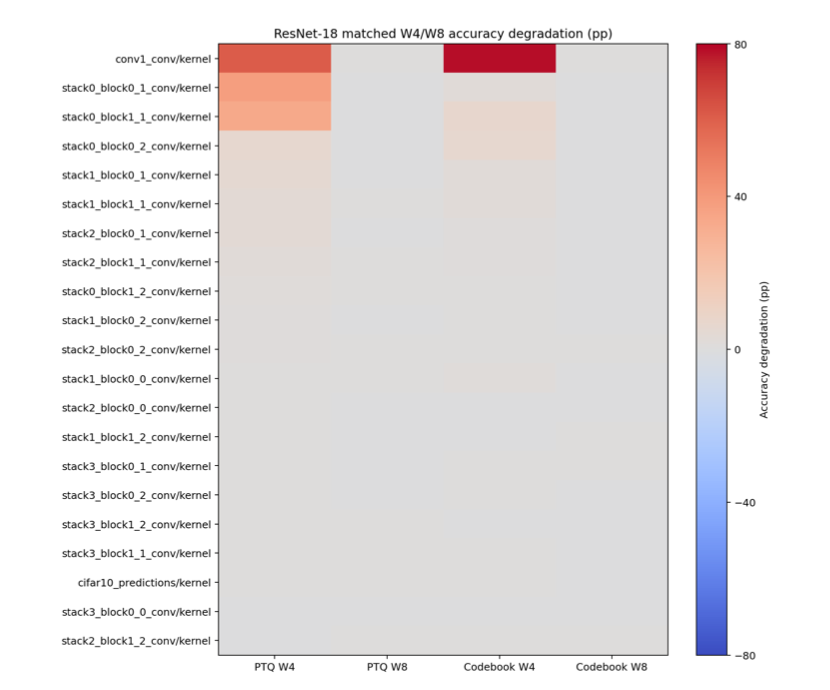
\includegraphics[width=\linewidth,height=.67\textheight,keepaspectratio]{resnet18_w4_w8_heatmap_from_report4.png}
\par\scriptsize\textbf{Colour range: $\pm80$ pp}
\column{.50\textwidth}
\begin{block}{Three most sensitive at W4}
\scriptsize
\begin{enumerate}
  \item \textbf{First convolution}\newline 78.62 pp codebook; 60.65 pp PTQ
  \item \textbf{Stack 0, block 0, conv 1}\newline 37.72 pp PTQ
  \item \textbf{Stack 0, block 1, conv 1}\newline 33.19 pp PTQ
\end{enumerate}
\end{block}
\begin{alertblock}{Explanation}
\scriptsize The common $\pm80$-pp scale exposes the extreme early-kernel losses; the smaller effects appear pale. At W8, every isolated loss is at most 0.53 pp.
\end{alertblock}
\end{columns}
\takeaway{The W4 failure is strongly localized to early kernels, especially the first convolution.}
\end{frame}

\begin{frame}{DistilBERT: tensor sensitivity}
\begin{columns}[c,onlytextwidth]
\column{.62\textwidth}\centering
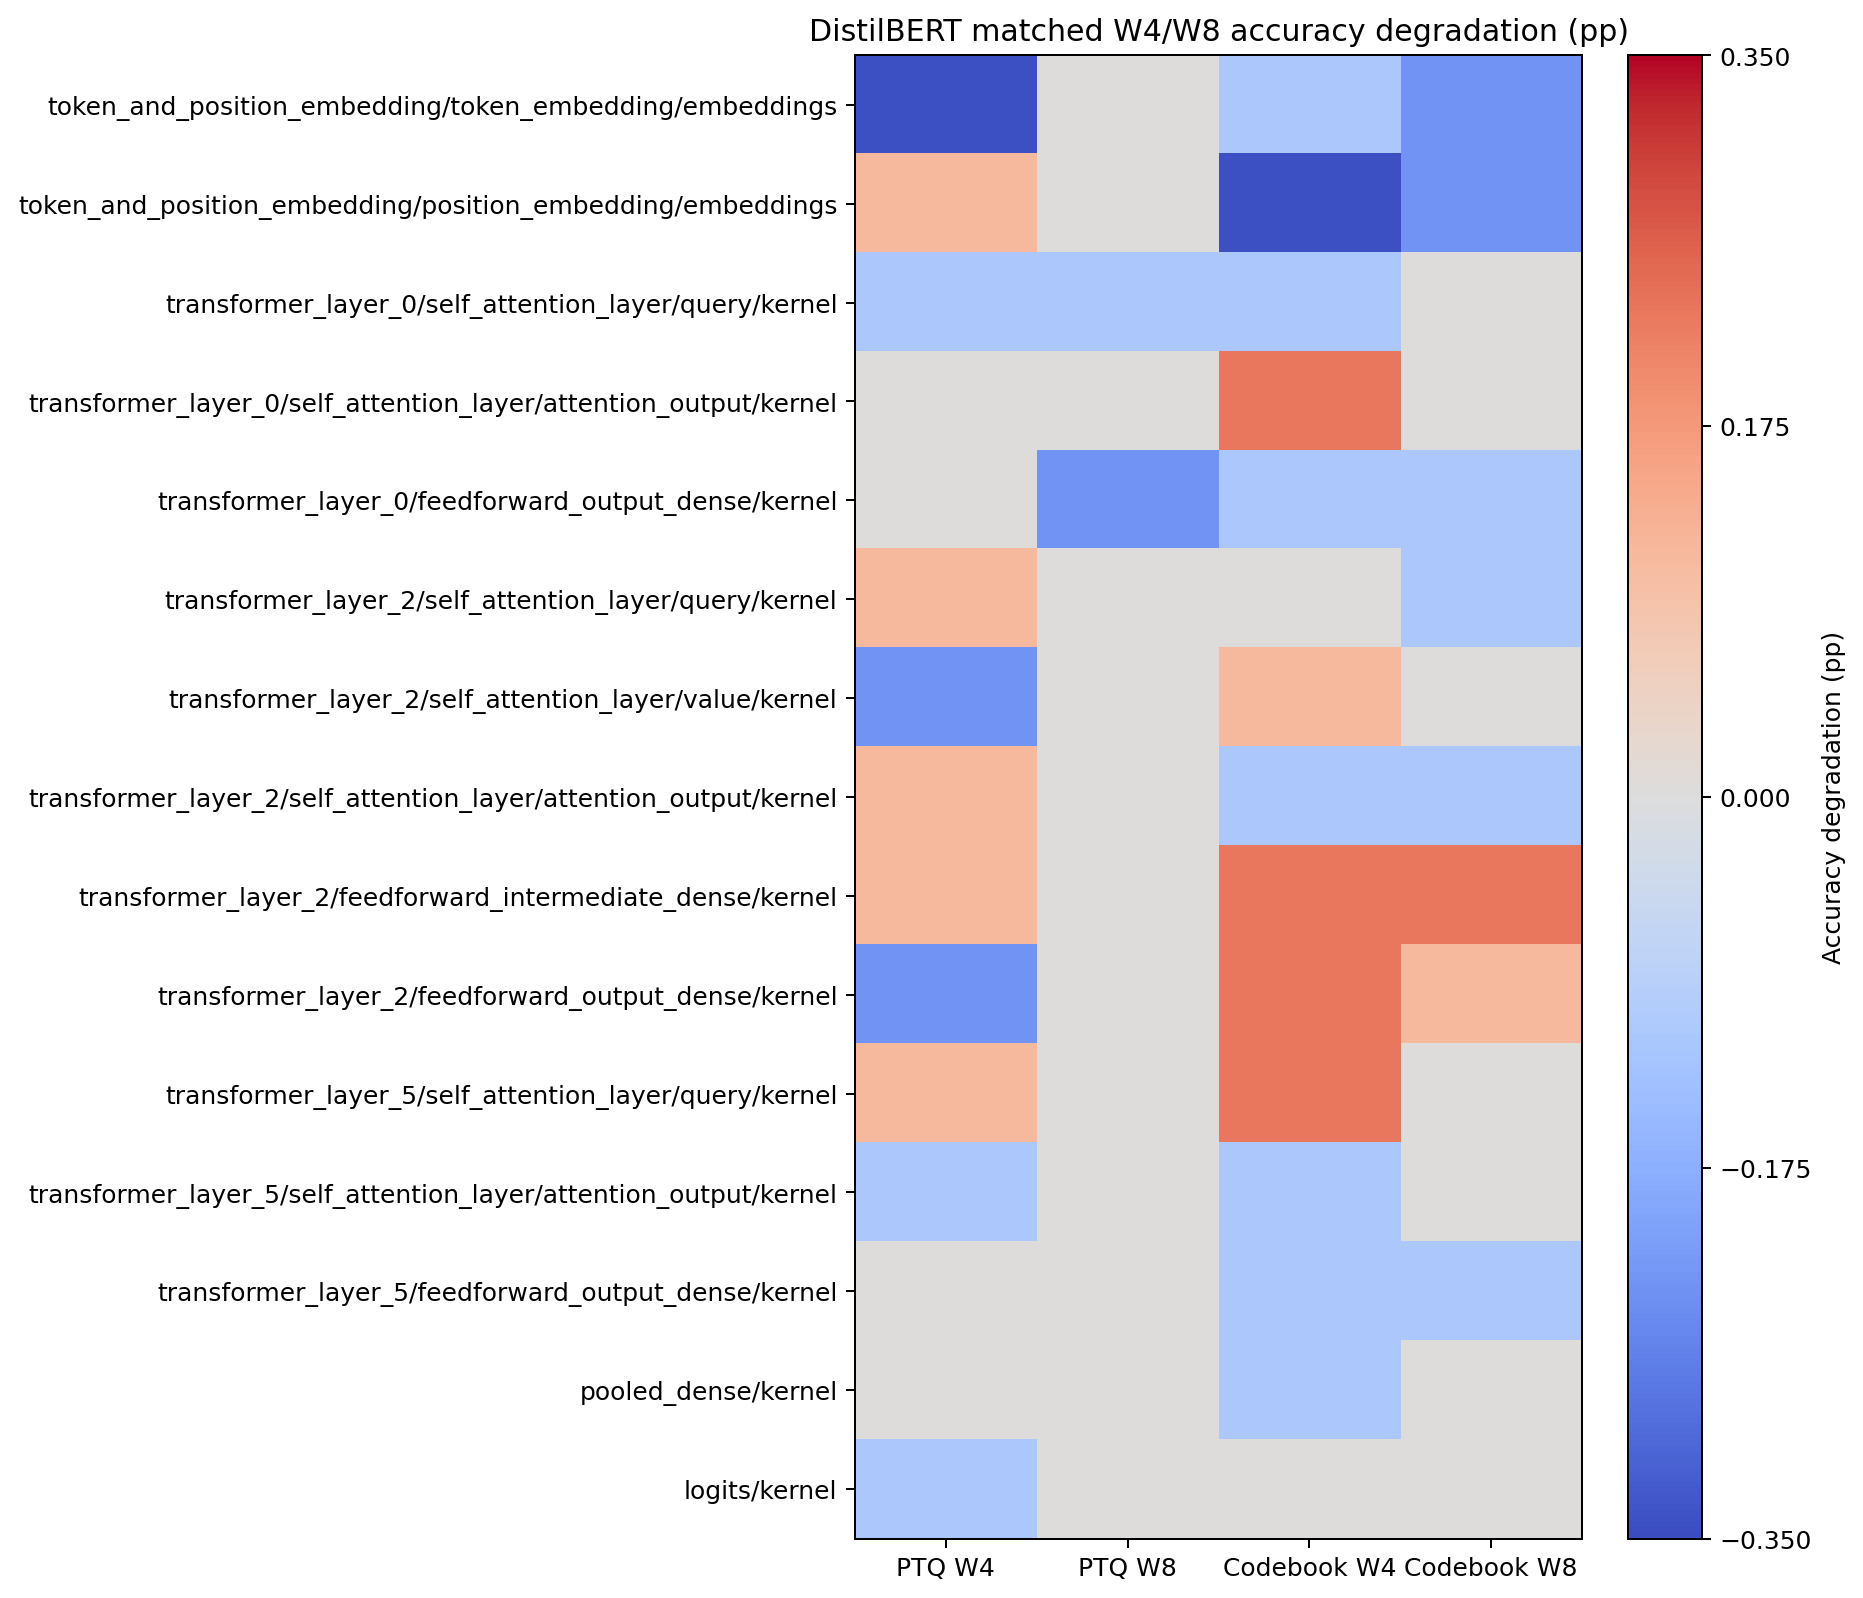
\includegraphics[width=\linewidth,height=.62\textheight,keepaspectratio]{distilbert_w4_w8_layer_sensitivity.png}
\par\scriptsize\textbf{Colour range: $\pm0.35$ pp}
\column{.36\textwidth}
\begin{block}{Three most sensitive at W4}
\scriptsize Codebook losses; tied at 0.229 pp and ordered by prediction disagreement:
\begin{enumerate}
  \item Layer 2 intermediate FFN
  \item Layer 0 attention output
  \item Layer 2 output FFN
\end{enumerate}
\end{block}
\begin{alertblock}{Explanation}
\scriptsize Effects are small and distributed across attention and feed-forward tensors. W4 covers 15 of 40 tensors.
\end{alertblock}
\end{columns}
\takeaway{No sampled tensor shows a ResNet-like collapse; the small effects must not be read as statistical equivalence.}
\end{frame}

\begin{frame}{ViT-B/16: module sensitivity}
\begin{columns}[c,onlytextwidth]
\column{.62\textwidth}\centering
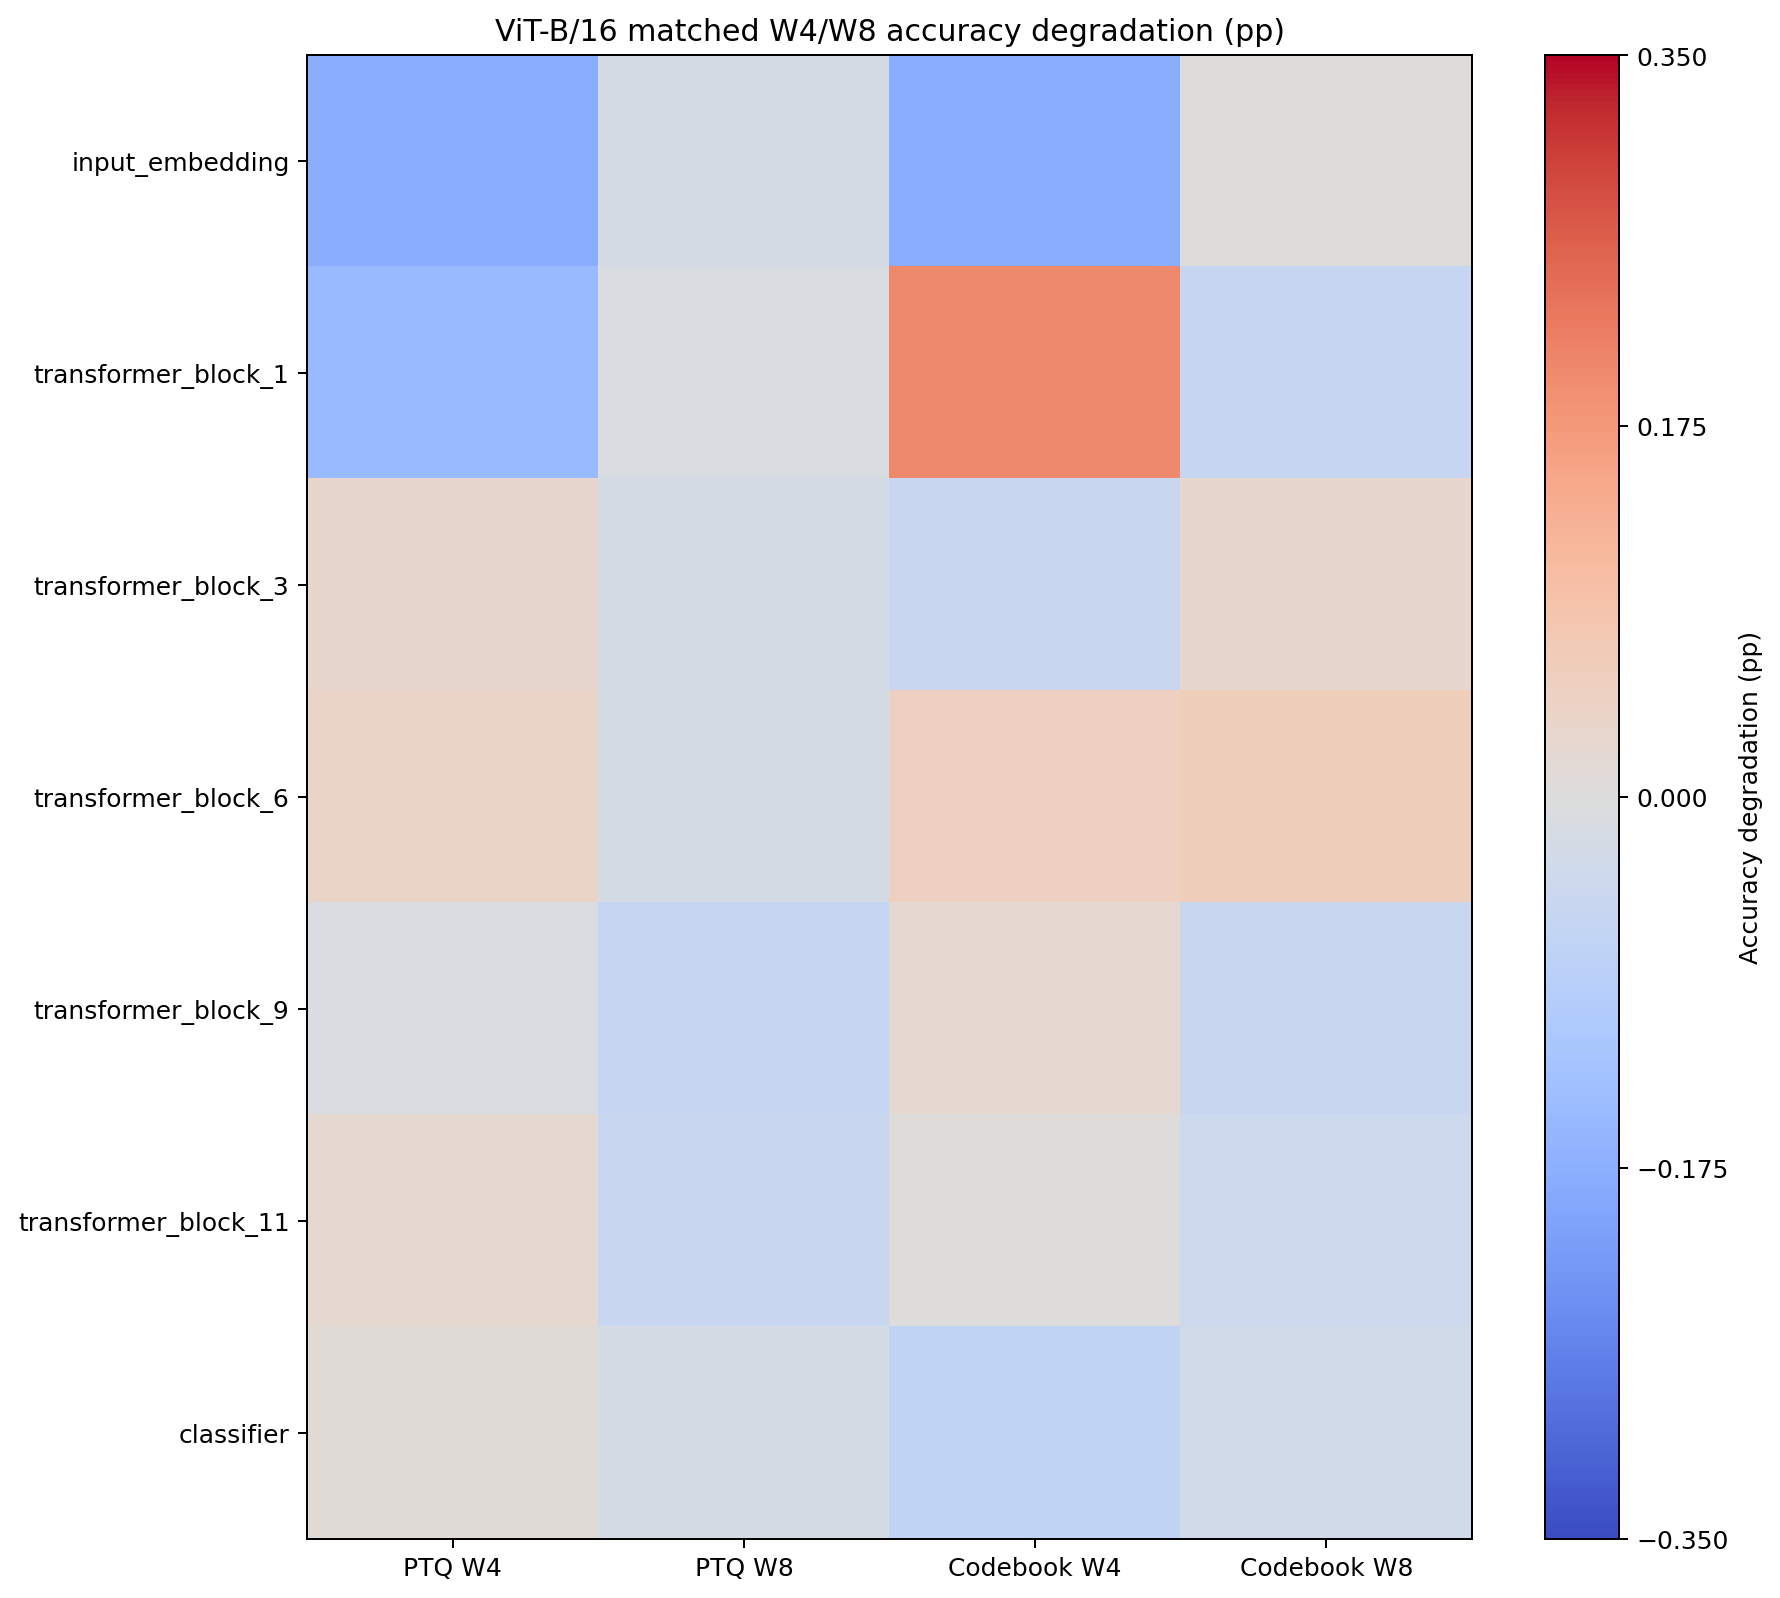
\includegraphics[width=\linewidth,height=.62\textheight,keepaspectratio]{vit_w4_w8_module_sensitivity_heatmap.png}
\par\scriptsize\textbf{Colour range: $\pm0.35$ pp}
\column{.36\textwidth}
\begin{block}{Three most sensitive at W4}
\scriptsize
\begin{enumerate}
  \item \textbf{Transformer block 1}\newline 0.20 pp codebook
  \item \textbf{Transformer block 6}\newline 0.05 pp codebook; 0.04 pp PTQ
  \item \textbf{Transformer block 3}\newline 0.03 pp PTQ
\end{enumerate}
\end{block}
\begin{alertblock}{Explanation}
\scriptsize The largest sampled effect occurs early, but all seven W4 module effects stay within $\pm0.20$ pp.
\end{alertblock}
\end{columns}
\takeaway{Overall: W8 is robust across these checkpoints; lower-bit accuracy is model- and method-dependent. ResNet's W4 failure concentrates in early kernels, while the sampled transformer units remain close to FP32.}
\end{frame}

\begin{frame}{Experiment 5: does W8 sensitivity predict W4? (RQ4)}
\begin{columns}[c,onlytextwidth]
\column{.57\textwidth}
\centering
\scriptsize
\begin{tabular}{llrrr}
\toprule
Model & Method & Units & $\rho$ & $p_{\mathrm{perm}}$\\
\midrule
ResNet-18 & PTQ & 21 & $-0.094$ & 0.68527\\
ResNet-18 & Codebook & 21 & $-0.292$ & 0.19867\\
DistilBERT & PTQ & 15 & 0.143 & 0.61139\\
\textbf{DistilBERT} & \textbf{Codebook} & \textbf{15} & \textbf{0.693} & \textbf{0.00551}\\
ViT-B/16 & PTQ & 7 & $-0.321$ & 0.49762\\
ViT-B/16 & Codebook & 7 & $-0.357$ & 0.44444\\
\bottomrule
\end{tabular}
\vspace{2mm}

\begin{beamercolorbox}[wd=\linewidth,sep=1.2mm,rounded=true]{block body}
\scriptsize
$\rho$: Spearman correlation between the W8 and W4 sensitivity rankings.\\[1mm]
$p_{\mathrm{perm}}$: permutation-test probability of observing an association this strong if the rankings are unrelated.
\end{beamercolorbox}
\column{.41\textwidth}
\begin{block}{One positive result}
\centering
\normalsize DistilBERT codebook\\[1mm]
\textcolor{TUIl-orange}{\bfseries $\rho=0.693$}\\
\textcolor{TUIl-orange}{\bfseries $p_{\mathrm{perm}}=0.00551$}
\end{block}
\begin{alertblock}{Interpretation}
\scriptsize A significant positive rank association was observed for the tested DistilBERT codebook subset. The other five tests provide insufficient evidence of transfer.
\end{alertblock}
\end{columns}
\takeaway{RQ4: General W8-to-W4 ranking transfer was not established.}
\end{frame}

\begin{frame}{Comparison: observed pattern and interpretation boundary}
\small
\begin{tabular}{>{\bfseries}m{26mm} m{31mm} m{31mm} m{31mm}}
\toprule
 & ResNet-18 & DistilBERT & ViT-B/16\\
\midrule
W8 & near baseline & near baseline & near baseline\\
W4 & severe collapse & within 0.6 pp & within 0.6 pp\\
Codebook edge & no at W4 & large at W2--W3 & very large at W3\\
Sensitive region & early kernels & scattered tensors & selected modules\\
\bottomrule
\end{tabular}
\vspace{3mm}
\begin{columns}[T,onlytextwidth]
\column{.475\textwidth}
\begin{block}{W8 headline}\centering
\normalsize\textbf{$\leq0.59$ pp loss}\\[-1mm]
\small approximately $4\times$ estimated compression
\end{block}
\column{.475\textwidth}
\begin{block}{Transformer W4 headline}\centering
\normalsize\textbf{within $0.6$ pp}\\[-1mm]
\small approximately $7.9\times$ estimated compression
\end{block}
\end{columns}
\vspace{1mm}
\begin{center}\scriptsize These are checkpoint- and pipeline-specific observations; training and quantizer differences prevent an architecture-only conclusion.\end{center}
\takeaway{The strongest defensible claim concerns these three evaluated configurations, not transformers versus CNNs in general.}
\end{frame}

\section{Conclusion}
\begin{frame}{Conclusions: answers to the research questions}
\begin{columns}[T,onlytextwidth]
\column{.49\textwidth}
\begin{block}{RQ1: How do bit width and method affect accuracy and storage?}
\scriptsize Compression followed bit width (about $4\times$ at W8 and $7.9\times$ at W4), while accuracy depended on the checkpoint and method; codebook retained more low-bit accuracy in selected DistilBERT and ViT cases.
\end{block}
\vspace{1mm}
\begin{block}{RQ3: Which units are most sensitive?}
\scriptsize ResNet-18's W4 damage concentrated in early kernels, especially \texttt{conv1}; the sampled DistilBERT tensors and ViT modules produced only small isolated accuracy changes.
\end{block}

\column{.49\textwidth}
\begin{block}{RQ2: How do the checkpoints respond at W4 and W8?}
\scriptsize At W8, all three checkpoints remained within 0.59 pp of FP32; at W4, ResNet-18 collapsed to 11.56\% PTQ and 8.43\% codebook, while DistilBERT and ViT stayed within 0.6 pp.
\end{block}
\vspace{1mm}
\begin{block}{RQ4: Does the W8 sensitivity ranking transfer to W4?}
\scriptsize General transfer was not established; only DistilBERT codebook was significant ($\rho=0.693$, permutation $p=0.00551$, Bonferroni-adjusted $p=0.03306$).
\end{block}
\end{columns}
\end{frame}

\begin{frame}{Selected references}
\scriptsize
\begin{columns}[T,onlytextwidth]
\column{.475\textwidth}
\begin{enumerate}
  \item K. He et al., ``Deep Residual Learning for Image Recognition,'' CVPR, 2016.
  \item A. Vaswani et al., ``Attention Is All You Need,'' NeurIPS, 2017.
  \item V. Sanh et al., ``DistilBERT,'' arXiv:1910.01108, 2019.
  \item A. Dosovitskiy et al., ``An Image Is Worth 16x16 Words,'' ICLR, 2021.
\end{enumerate}
\column{.475\textwidth}
\begin{enumerate}\setcounter{enumi}{4}
  \item B. Jacob et al., ``Quantization and Training of Neural Networks,'' CVPR, 2018.
  \item R. Krishnamoorthi, ``Quantizing Deep Convolutional Networks,'' arXiv:1806.08342, 2018.
  \item R. M. Gray, ``Vector Quantization,'' IEEE ASSP Magazine, 1984.
  \item S. P. Lloyd, ``Least Squares Quantization in PCM,'' IEEE TIT, 1982.
\end{enumerate}
\end{columns}
\vspace{2mm}
\begin{center}\scriptsize Statistical and transformer-PTQ references are listed in the accompanying report.\end{center}
\end{frame}

\lastframe{Questions?}{Thank you}{TU Ilmenau campus}

\appendix
\begin{frame}{Backup: BatchNorm hypothesis for the ResNet W4 collapse}
\begin{center}
\resizebox{.88\textwidth}{!}{%
\begin{tikzpicture}[node distance=8mm]
  \node[orangecard,minimum width=33mm] (round) {W4 rounding in\\early convolutions};
  \node[process,right=of round,minimum width=34mm] (shift) {possible activation-\\distribution shift};
  \node[card,right=of shift,minimum width=35mm] (bn) {saved FP32 BatchNorm\\statistics at inference};
  \node[orangecard,right=of bn,minimum width=34mm] (prop) {possible downstream\\error amplification};
  \draw[floworange,dashed] (round)--(shift);
  \draw[floworange,dashed] (shift)--(bn);
  \draw[floworange,dashed] (bn)--(prop);
\end{tikzpicture}}
\end{center}
\vspace{3mm}
\begin{columns}[T,onlytextwidth]
\column{.475\textwidth}
\begin{block}{Recorded policy}
\small
\begin{itemize}
  \item BatchNorm scale, offset, moving mean and variance remain FP32.
  \item Inference uses \emph{training=False}.
  \item No folding, recalibration, bias correction, equalization or adaptive rounding.
\end{itemize}
\end{block}
\column{.475\textwidth}
\begin{alertblock}{What is established}
\small
\begin{itemize}
  \item Quantizing \emph{conv1} alone causes the largest W4 loss.
  \item BatchNorm mismatch is a plausible mechanism, but it was not isolated or tested.
  \item The study makes no claim that recalibration would recover accuracy.
\end{itemize}
\end{alertblock}
\end{columns}
\takeaway{The location of the failure is measured; its causal mechanism remains unresolved.}
\end{frame}
\end{document}
